\documentclass[a4paper,11pt]{article}


\def\prob{\mathbb{P}}
\def\ind{\mathbb{I}}
\def\expec{\mathbb{E}}
\def\Cov{\mathrm{Cov}}
\def\Var{\mathrm{Var}}

\usepackage{amsmath, amssymb, amsfonts, amsthm,graphicx,float,multirow,fullpage,cool,enumitem}

\begin{document}
\title{Calculating a Locus of Saddle-Node Bifurcations of Periodics with $\texttt{AUTO}$}
\author{Joe McKenna}
\date{}
\maketitle

\section*{Summary}

An example system that undergoes a saddle-node bifurcation of periodics is analyzed. Relations between parameters and variables for which the system undergoes the bifurcation are derived and accurately predict \texttt{AUTO} calculations. An explanation of using \texttt{AUTO} to continue the saddle-node bifurcation of periodics in two parameters is given. The general approach is to locate a Hopf bifurcation on a stationary branch, locate a saddle-node bifurcation of periodics on the periodic branch emanating from the Hopf bifurcation, and continue the saddle-node bifurcation of periodics in two parameters. If the Hopf bifurcation or saddle-node bifurcation of periodics is known \emph{a priori}, the first one or two steps, resp., are not necessary to complete the third.

\section*{Bifurcation Analysis of Example System}

Consider the ODE system in polar coordinates
\begin{align}\label{1}
\left\{\begin{array}{ll}
\dot{r}&=r(r(b-r)-c)\text{ for }b>0\\
\dot{\theta}&=r.
\end{array}\right.
\end{align}
It can be seen from the graph of $\dot{r}$ vs. $r$  that~\eqref{1} undergoes a saddle-node bifurcation of periodics. An explanation is provided below.
\begin{center}
\begin{figure}[H]
  \centering
    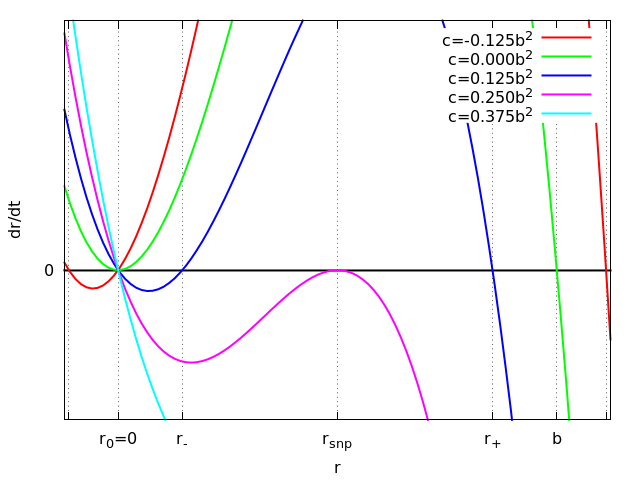
\includegraphics[scale=.49]{gnuplot/fig1.png}
 \caption{$\dot{r}$ vs. $r$ for~\eqref{1}.}
\label{fig1}
\end{figure}
\end{center}
The stationary radii of~\eqref{1}, given by $\dot{r}=0$, are $r_0=0$ and the roots that result from translating $r(b-r)$ down by $c$, that is, $r_{\pm}=\frac{b}2\pm\sqrt{\frac{b^2}4-c}$. Note also, since $\dot{\theta}\geq0$, the flow everywhere in the $xy$-plane except at the origin is counter-clockwise.\vspace{3mm}

\noindent
For $0<c<\frac{b^2}4$, there are three distinct stationary radii $0=r_0<r_-<r_+$ for which $\dot{r}(r_0)$, $\dot{r}(r_+)<0$ and $\dot{r}(r_-)>0$ (Fig 1, blue), so in the $xy$-plane,~\eqref{1} has a stable equilibrium point $(0,0)$ surrounded by unstable and stable limit cycles with radii $r_-<r_+$, resp.\vspace{3mm}

\noindent
As $c\uparrow\frac{b^2}4$, $r_+$ and $r_-$ collide at $r_{snp}=\frac{b}2$, for which $\dot{r}(r_{snp})=0$ and $\ddot{r}(r_{snp})<0$ (Fig 1, purple), so in the $xy$-plane,~\eqref{1} has a stable equilibrium point $(0,0)$ surrounded by a semi-stable (attracts for initial conditions with $r\geq r_{snp}$, repels otherwise) limit cycle with radius $r_{snp}$.\vspace{3mm}

\noindent
For $c>\frac{b^2}4$, the only real solution to $\dot{r}=0$ is $r_0=0$, for which $\dot{r}(r_0)<0$ (Fig 1, cyan), so in the $xy$-plane,~\eqref{1} has as its only equilibrium the stable equilibrium point $(0,0)$.\vspace{3mm}

\noindent
We have shown that a saddle-node bifurcation of periodics occurs at $(c_{snp},r_{snp})=(\frac{b^2}{4},\frac{b}2$). It can also be seen from Figure 1 that $(0,0)$ becomes stable as it gives rise to an unstable limit cycle when $c$ increases past zero, that is, the system undergoes a subcritical Hopf bifurcation at $(c,r)=(0,0)$. Below are system phase portraits corresponding to the $c$ values in Figure 1.\vspace{3mm}

\begin{center}
\begin{figure}[H]
  \centering
    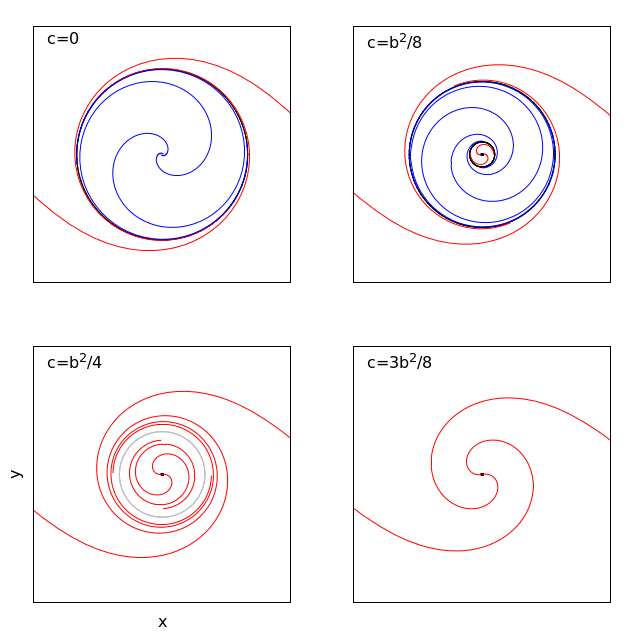
\includegraphics[scale=.5]{gnuplot/fig2.png}
 \caption{Phase portraits corresponding to Figure 1. The $x$ and $y$ range of each graph is $3b$ and all flows are counter-clockwise.}
\label{fig2}
\end{figure}
\end{center}

\noindent
Now that we have an analytic relation in $(b,c)$ and $(c,r=\max y)$ for which the system undergoes a saddle-node bifurcation of periodics, we could graph the bifurcation locus in the $bc$-plane and the $cy$-plane by simply plotting $c=\frac{b^2}4$ and $y=\sqrt{c}$, resp., but we will use \texttt{AUTO} to generate these graphs.\vspace{3mm}

\noindent
Figure 3 is the bifurcation diagram of~\eqref{1} with $c$ as a bifurcation parameter in a neighborhood of zero. We will explain how the data plotted in the diagram were generated using \texttt{AUTO} and how they were used to calculate the locus of saddle-node bifurcations of periodics.\vspace{3mm}

\begin{center}
\begin{figure}[H]
  \centering
    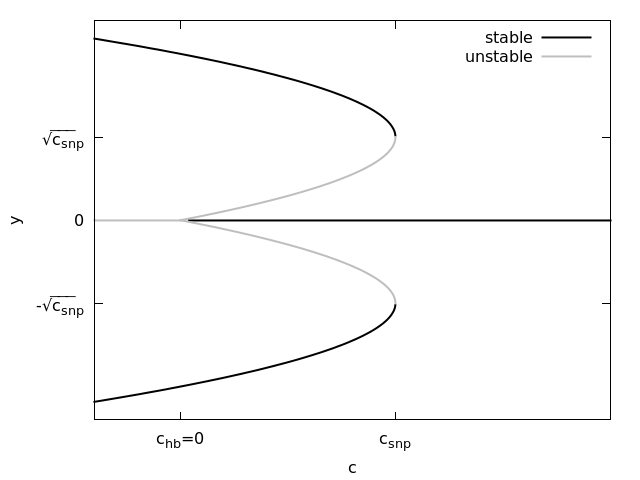
\includegraphics[scale=.5]{gnuplot/fig3.png}
 \caption{Bifurcation diagram.}
\label{fig3}
\end{figure}
\end{center}

\section*{Using \texttt{AUTO}}

\noindent
For each run, \texttt{AUTO} expects two files, one to specify the system equations and initial conditions and one to specify the constants that dictate the program's behavior.

\subsection*{The Equations File}

\noindent
For this example, the system equations and initial conditions appear in \texttt{snp.f90}, in the two functions \texttt{FUNC} and \texttt{STPNT}, resp. The values of $x,y,b$, and $c$ are referred to as \texttt{U(1)}, \texttt{U(2)}, \texttt{PAR(1)}, and \texttt{PAR(2)}, resp. The equations~\eqref{2} appearing in \texttt{FUNC} are derived from~\eqref{1} as follows. Transforming~\eqref{1} into rectangular coordinates, we write
\begin{align*}
\left(\begin{array}{cc}
x&y\\
-y&x\\
\end{array}\right)
\begin{pmatrix}\dot{x}\\\dot{y}\end{pmatrix}&=
r^2\begin{pmatrix}p-c\\r\end{pmatrix}
\end{align*}
where $p(r)=r(b-r)$, since $\dot{r}=\frac1r\begin{pmatrix}x&y\end{pmatrix}\begin{pmatrix}\dot{x}&\dot{y}\end{pmatrix}^T$ and $\dot{\theta}=\frac1{r^2}\begin{pmatrix}-y&x\end{pmatrix}\begin{pmatrix}\dot{x}&\dot{y}\end{pmatrix}^T$ for $r=\sqrt{x^2+y^2}$. Multiplying by the inverse of the lefthand side matrix and rearranging, we get
\begin{align}\label{2}
\begin{pmatrix}\dot{x}\\\dot{y}\end{pmatrix}&=
\left(\begin{array}{cc}
x&-y\\
y&x\\
\end{array}\right)\begin{pmatrix}p-c\\r\end{pmatrix}\nonumber\\
\begin{pmatrix}\dot{x}\\\dot{y}\end{pmatrix}&=\left(\begin{array}{cc}
p-c&-r\\
r&p-c\\
\end{array}\right)\begin{pmatrix}x\\y\end{pmatrix}.%\\
%\dot{\vec{z}}&=(\text{diag}(p(z)-c)+rS)\vec{z}\hspace{3mm}
\end{align}
%where $S=\left(\begin{array}{cc}0&-1\\1&0\end{array}\right)$. In general, for $\dot{r}=f$ and $\dot{\theta}=g$, $\begin{pmatrix}\dot{x}\\\dot{y}\end{pmatrix}=\left(\begin{array}{cc}f/r&-g\\g&f/r\end{array}\right)\begin{pmatrix}x\\y\end{pmatrix}$. Don't let the matrices fool you.. this is a nonlinear system.
The variables and parameters initialized in \texttt{STPNT} are chosen to first locate a Hopf bifurcation on a branch of stationary solutions. Knowing that for $b>0$, a Hopf bifurcation occurs as $c$ increases past zero at the equilibrium point $(x,y)=(0,0)$, we initialize $b=1$, $c=-0.1$, $x=0$, and $y=0$, and intend to continue the solution $(0,0)$ with $c$ increasing to $0.5$. After locating the Hopf bifurcation, we continue in $c$ the periodic solutions that arise from it to locate a saddle-node bifurcation of periodics. Finally, we continue in $b$ and $c$ the saddle-node bifurcation of periodics.

\subsection*{The Constants Files}

\noindent
For this example, the constants that dictate the program's behavior appear in three different files \texttt{c.snp.ss}, \texttt{c.snp.ps}, and \texttt{c.snp.snp} (\texttt{AUTO} expects each constants file to begin with the \texttt{c.} prefix) for computing stationary solutions, periodic solutions, and saddle-nodes of periodics, resp. The full meaning of each constant is explained in Chapter 10 of the \texttt{AUTO} documentation (\texttt{auto.pdf}) but important values for the current example are explained here.\vspace{3mm}

\noindent
In \texttt{c.snp.ss}, the value \texttt{IPS=1} (problem specification index) indicates that a stationary solution is to be continued and Hopf bifurcations are to be detected. The value \texttt{IRS=0} (restart index) indicates that the continuation is to start from the initial conditions specified in \texttt{snp.f90}. The value \texttt{ICP=['c']} (continuation parameter index) indicates that $c$ is the continuation parameter. The value \texttt{UZSTOP=\{'c':.5\}} indicates that continuation should stop when $c$ reaches the value $0.5.$ Note there are other ways to stop continuation such as specifying a maximum number of steps with \texttt{NMX}, maximum number of bifurcations with \texttt{MXBF}, maximum number of bifurcations of a specific type with \texttt{SP} (for example, \texttt{SP=['HB1']} would stop the continuation at the first Hopf bifurcation), etc.\vspace{3mm}

\noindent
In \texttt{c.snp.ps}, the value \texttt{IPS=2} indicates that a periodic solution is to be continued. The value \texttt{ILP=1} (limit point index) turns on detection of limit points, which allows us to locate the saddle-node bifurcation of periodics. The value \texttt{ICP=['c','PERIOD']} indicates that $c$ and period are continuation parameters. By default, \texttt{AUTO} records maximum values of the system variables when continuing periodic solutions. Setting the value \texttt{IPLT=-2} indicates that the minimum values of $y=\texttt{U(2)}$ are also to be recorded. The value \texttt{THL=\{'PERIOD':0.0\}} neglects period in determining the continuation stepsize to avoid problems near homoclinic orbits, a standard precaution taken when continuing periodic solutions.\vspace{3mm}

\noindent
In \texttt{c.snp.snp}, the value \texttt{ICP=['c','b','PERIOD']} indicates that $c$, $b$, and period are continuation parameters. The value \texttt{ISW=2} (branch switching index) allows \texttt{AUTO} to compute a locus of saddle-node bifurcations of periodics.

\subsection*{The \text{AUTO} Script}

\noindent
The commands that generate the bifurcation diagram data are summarized in the script \texttt{snp.auto}. They can be run all-at-once from a UNIX command line with \texttt{auto snp.auto} or step-by-step from the \texttt{AUTO} command line with \texttt{demofile('snp.auto')}. Here, we explain the effect of each command in \texttt{snp.auto}.\vspace{3mm}

\noindent
First, the stationary branch is stored in the bifurcation diagram object \texttt{ss} by running \texttt{ss=run(e} \texttt{='snp',c='snp.ss')}. The arguments \texttt{e='snp'} and \texttt{c='snp.ss'} specify the names of the equations and constants file, resp. In the terminal output from this command, you should see that \texttt{AUTO} identified a Hopf bifurcation and labelled it 2. Next, the periodic branch is stored in \texttt{ps} by running \texttt{ps=run(ss('HB1'),c='snp.ps')}. The argument \texttt{ss('HB1')} overrides the value of \texttt{IRS} in the constants file \texttt{c.snp.ps} and instructs \texttt{AUTO} to continue from the first Hopf bifurcation located on the stationary branch \texttt{ss}. In the terminal output from this command, you should see that \texttt{AUTO} identified a saddle-node bifurcation of periodics and labelled it 4. Next, starting data for continuing the saddle-node bifurcation of periodics is stored in \texttt{snpstart} by running \texttt{snpstart=run(ps('LP1'),c='snp.snp')}. Last, the locus of saddle-node bifurcations of periodics is stored in \texttt{snp} by running \texttt{snp=merge(run(snpstart)+run(snpstart,DS='-'))}. This command merges continuations of the saddle-node bifurcation of periodics for both increasing and decreasing values of continuation parameters. The continuation for solely increasing or decreasing values of continuation parameters could be stored in \texttt{snp} by running \texttt{snp=run(snpstart)} or \texttt{snp=run(snpstart,DS='-')}, resp.\vspace{3mm}

\noindent
The data from each branch are combined and saved in the files \texttt{b.snp}, \texttt{s.snp}, and \texttt{d.snp} in a format explained in the \texttt{AUTO} documentation by running \texttt{save(ss+ps+snp,'snp')}. The temporary files created by \texttt{AUTO} are deleted by running \texttt{clean}.

\section*{Plotting the Data}

\noindent
The locus of saddle-node bifurcations of periodics is plotted in Figure 4. The data, including values for $b$, $c$, $\min y$, $\max y$, $\max x$, and period, appear in both \texttt{b.snp} and the last data block of \texttt{tex/gnuplot/unstable.dat}. While using \texttt{AUTO}, any stored bifurcation diagram object, say \texttt{x}, can be graphed with \texttt{PyPlot} by running \texttt{plot(x)} from the \texttt{AUTO} command line. Also, the \texttt{AUTO} documentation describes a few methods for exporting data.\vspace{3mm}

\noindent
I've written a small program \texttt{cleanData} that reformats the data in \texttt{b.snp} into a number of data blocks in two files \texttt{tex/gnuplot/stable.dat} and \texttt{tex/gnuplot/unstable.dat}. Each data block corresponds to a connected portion of a branch with the same stability. The source \texttt{cleanData.cpp} may be modified for a different project by recompiling it after changing the name of the input and output data files specfied in the source file. \vspace{3mm}

\noindent
The formats of \texttt{stable.dat} and \texttt{unstable.dat} are conducive to graphing with \texttt{gnuplot}. For example, the scripts that generated Figures 1 - 4, appearing in \texttt{tex/gnuplot/plot1.p} - \texttt{plot4.p}, use the two data files. These can be run in \texttt{tex/gnuplot} from a UNIX command line with \texttt{gnuplot plot.p} or from the \texttt{gnuplot} command line with \texttt{load 'plot.p'}. Also, the data plotted in Figure 2 were generated by integrating~\eqref{2} with \texttt{CVODE} by running \texttt{make} (requires \texttt{CVODE}) then \texttt{snp} in \texttt{tex/gnuplot/fig2data}.
\begin{center}
\begin{figure}[H]
  \centering
    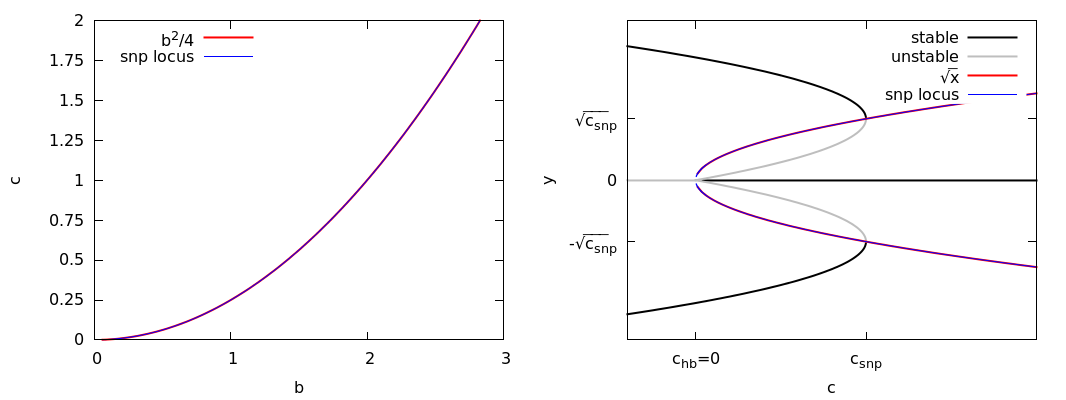
\includegraphics[scale=.4]{gnuplot/fig4.png}
 \caption{The locus of saddle-node bifurcations of periodics.}
\label{fig4}
\end{figure}
\end{center}

\end{document}
